\section{Results \& Discussion} \label{sec:results}
With our trained NDE, $q_{\phi}(\Omega, \mathcal{B}\given {\bfi X_i})$, we can
now evaluate the posterior $p(\Omega, \mathcal{B}\given\{\bfi X_i\})$ for
multiple galaxies using Eq.~\ref{eq:posterior}. 
In Fig.~\ref{fig:p_omega_x}, we present 
$p(\Omega, \mathcal{B}\given\{\bfi X_i\})$ for the 14,736 observed galaxies in
our NSA sample.
The contours mark the 68 and 95 percentiles of the distribution and we list the
median and $\pm1\sigma$ marginalized constraints on $\Omega_m$, $\sigma_8$, and
$S_8 = \sigma_8\sqrt{\Omega_m/0.3}$. 
The samples from $p(\Omega\given\{\bfi X_i\})$ are derived using Markov Chain
Monte Carlo (MCMC). 
We use the $\mathtt{emcee}$ sampler~\citep{foreman-mackey2013} with 1,000
walkers evaluated 36,000 iterations, discarding the first 5,000 iterations for
burn in.

\begin{figure}[ht]
\vskip 0.2in
\begin{center}
    \centerline{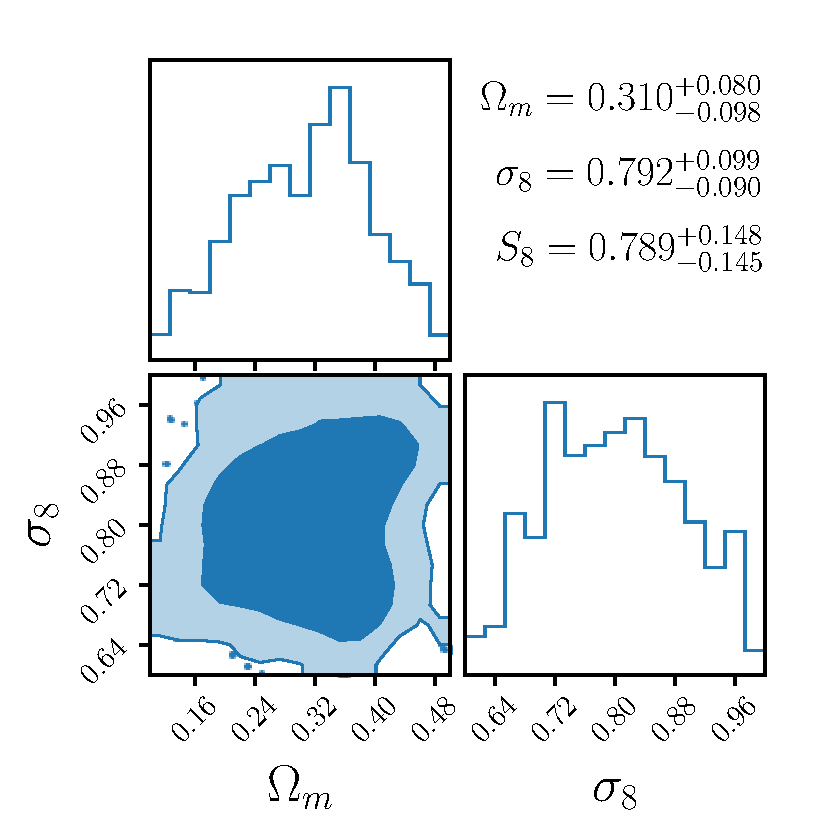
\includegraphics[width=0.9\columnwidth]{figs/p_oms8_x.pdf}}
    \caption{The posterior on $\Omega_m$ and $\sigma_8$ from the observed
    photometry of 14,736 NSA galaxies.
    The contours mark the 68 and 95 percentiles. 
    We place significant cosmological constraints from only the photometry of 
    galaxies. 
    }\label{fig:p_omega_x}
\end{center}
\vskip -0.2in
\end{figure}

Overall, we derive significant constraint on both $\Omega_m$ and $\sigma_8$: 
$\Omega_m = 0.310^{+0.080}_{-0.098}$ and $\Omega_m = 0.792^{+0.099}_{-0.090}$. 
Although, we also derive significant constraints on the hydrodynamical
parameters, we do not include them for clarity.  
Our cosmological constraints demonstrate that although the photometry of a
single galaxy does not contain a significant amount of cosmological
information, we can place significant cosmological constraints by combining the
information from 14,736 galaxies. 

Interestingly, our constraints can inform the latest tension between growth of
structure $S_8$ constraints from large-scale structure (LSS) and CMB
experiments. 
Low redshift LSS experiments find a significantly lower value of $S_8$ than CMB
experiments and has placed renewed scrutiny on the standard
$\Lambda$CDM cosmological model.
Our $S_8 = 0.789^{+0.148}_{-0.145}$ constraint is consistent with the lower LSS
$S_8$ values; however, it is not precise enough to competitive inform the
tension. 

A major caveat of our constraint is that our posterior assumes a galaxy
formation and a SED models. 
This assumption is more clearly expressed if we rewrite 
\begin{equation}
    p(\Omega, \mathcal{B}\given {\bfi X_i}) \propto p(\Omega, \mathcal{B}) \int     p(\theta^g_i \given {\bfi X_i})\, p(\Omega, \mathcal{B}\given \theta^g_i)\,
    {\rm d}\theta^g_i.
\end{equation}
$p(\theta^g_i\given\Omega, \mathcal{B})$, in our case, is the TNG simulation. 
Although TNG is a state-of-the-art hydrodynamical simulation, it makes specific
choices and assumptions for its subgrid approximations. 
Consequently, an alternative galaxy formation model would produce a
significantly different $p(\theta^g_i\given\Omega, \mathcal{B})$. 
For instance, \cite{hahn2019} found significantly discrepant $M_*$-star
formation rate relations in three state-of-the-art hydrodynamical
simulations.

Similarly, $p({\bfi X_i}\given\theta^g_i)$ is given by the SED model, which
also include a number of choices and assumptions. 
For instance, we use a dust model that assumes that dust is cospatial and
uniformly mixed. 
Yet, recent studies suggest that the dust-star geometry can be significantly
more complex and, thus, produce a wider range of attenuation
curves~\citep{narayanan2018a, hahn2021}. 
The SED model also does not sufficiently model nebular emission lines,
which may be significantly impact of photometry of emission ilne galaxies. 
Furthermore, the SED model assumes a fixed Chabrier IMF.  

Despite these major limitations, a key advantage of our approach is that we can
systematically choose subpopulations of galaxies that are the most robust to
the assumptions in the galaxy formation and SED models. 
For example, we can compare 
$p(\theta^g_i\given\Omega, \mathcal{B})$ across multiple galaxy formation
models and choose the galaxies that are consistently predicted by the models. 
We can take a similar approach for the SED modeling assumptions by selecting
galaxies without emission lines and  with limited dust attenuation (\eg~by
using infrared photometry). 
We can also identify galaxy populations with observationally constrained
IMFs~\citep{myers2013, smith2015a}.

Another key advantage is that our cosmological constraining power depends on
the number of galaxies we include. 
In this work, we selected $\sim$15,000 NSA galaxies using conservative noise
and color cuts.
They were from the NSA catalog, which only has $\sim$120,000 galaxies total.
Upcoming spectroscopic surveys such as the Dark Energy Spectroscopic
Survey~\citep[DESI;][]{desicollaboration2016, desicollaboration2016a,
abareshi2022} Bright Galaxy Survey~\citep[BGS;][]{hahn2022c} will observe 
{\em orders of magnitude} larger galaxy samples. 
With the millions of galaxies that they will observe, these surveys will
provide an enormous number of galaxies that we can analyze even if we restrict
our samples to galaxy populations robust to our modeling assumptions.
Furthermore, these upcoming galaxy samples will have spectra, in addition to
photometry, which will also provide more information per galaxy. 
